\documentclass[crop,tikz]{standalone}
\usetikzlibrary{backgrounds}
\colorlet{blue}{cyan}
\tikzset{
  inverted/.style = {
    color=white,
    background rectangle/.style={fill},
    show background rectangle
  }
}

\usepackage[european]{circuitikz}

\tikzset{>=latex}

\begin{document}
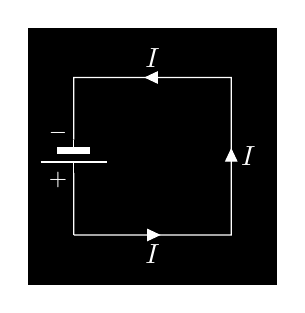
\begin{tikzpicture}[inverted,inverted]
  \draw (0,-1) to[battery2] ++(0,2)
    to[short,i<=$I$] ++(2,0)
    to[short,i<=$I$] ++(0,-2)
    to[short,i<=$I$] ++(-2,0);
  \node at (-0.2,-0.3) { \footnotesize $+$};
  \node at (-0.2,+0.3) { \footnotesize $-$};
\end{tikzpicture}
\end{document}
